\setcounter{step}{0}

\subsection{ Cestoviny }

\begin{ingredient}
  
      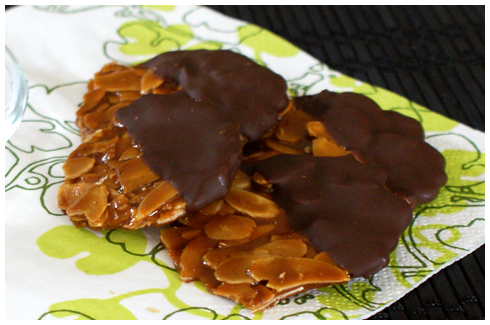
\includegraphics[height=5.5cm]{images/florentin}
  
  \def\portions{  }
  \textbf{ {\normalsize Ingrediencie (1 porcie):} }

  \begin{main}
      \item hokkaido, 150g na človeka
      \item ryža (Carnaroli, Arborigio ak nie je iná gulatozrnná sa tiež prežije), 75g na človeka
      \item msalo, 20g
      \item parmezán, 25g
      \item voda, 200ml
  \end{main}
  
\end{ingredient}
\begin{recipe}
\textbf{ {\normalsize Príprava:} }
\begin{enumerate}

  \item{Nakrájame tekvicu (150g/človeka) na 2 cm kocky.}
  \item{Tekvicu dáme variť do osolenej vody na 5 minút (čas meriame od kedy voda začne vrieť).}
  \item{Pridáme ryžu, občas premiešame a varíme cca 15 minút alebo až kým nebude ryža mäkká}
  \item{pri najhoršom dolejeme trochu vody aby nám to nezhorelo.}
  \item{V tomto štádiu by mala byť v hrnci kašovitá ale relatívne riedka}
  \item{hmota (proste tak aby sa mam to nepripalilo).}
  \item{Vypneme sporák, pridáme maslo a nastrúhaný parmezán.}
  \item{Rozmiešame a môžme podávať.}
  \item{Môžme dochutiť soľou, provensálskymi bylinkami, čiernym korením alebo osmaženými šalviovými lístkami.}

\end{enumerate}
\end{recipe}

\begin{notes}
  
\end{notes}	
\clearpage
